\documentclass{scribe}
\usepackage{float}

%====================================================================
%====================================================================
% IMPORTANT: PLEASE UPDATE THE LECTURE INFORMATION BELOW:
\setcounter{lecture}{12} % Lecture number here, from The Big Table on Canvas
\renewcommand{\lectureTitle}{Modes of operation: CTR, OFB, ECB. Pseudorandom permutations (PRP), CBC.}
\renewcommand{\lecturer}{Mahdi Cheraghchi}
\renewcommand{\scribe}{Yi-Wen Tseng}
\renewcommand{\lectureDate}{February 15, 2023} % Date of the lecture
%====================================================================
%====================================================================

\begin{document}

\maketitle

%=============================================================================
%=============================================================================

\section{Counter Mode (CTR)}

\begin{figure}[h]
  \centering
  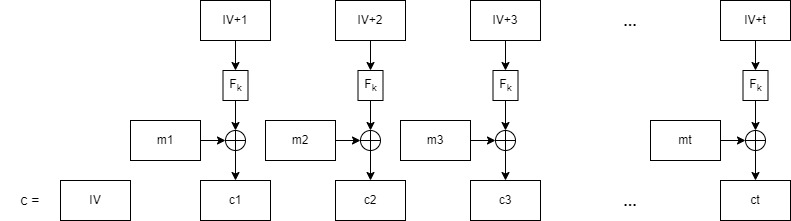
\includegraphics[width=0.8\textwidth]{ctr.jpg}
  \caption{CTR Mode Encryption}
\end{figure}
By using CTR, we can now encrypt messages of various lengths: message space $M$:$\{0,1\}^{*}$. Additionally, if $F$ is PRF (pseudorandom function), then CTR is CPA secure.
\\
\\\underline{\textbf{Proof:}} Every Input to $F$ across the entire CPA game is distinct, with a very negligible probability to be the same. Therefore, all output of $F$ will \emph{look like} truly random and independent.
\\
\\Advantages of using CTR:
\begin{itemize}
  \item Simple and satisfy CPA secure
  \item Fast and efficient because it can be computed in parallel
  \item No need for padding (we can just trim the output of $F$ to fit the last message block size)
\end{itemize}

%=============================================================================
%=============================================================================

\section{Output Feedback Mode (OFB)}
\begin{figure}[H]
  \centering
  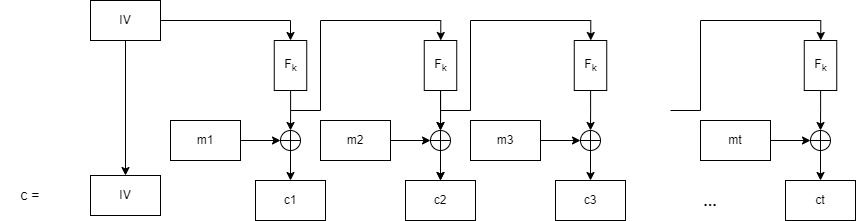
\includegraphics[width=0.8\textwidth]{ofb.jpg}
  \caption{OFB Mode Encryption}
\end{figure}
\begin{itemize}
    \item OFB is random by the chain, which is independent of message, not by counter.
    \item OFB is also CPA secure because it essentially does not have repeated input to $F$ (happen with negligible probability).
    \item OFB can increase security. 
    \begin{itemize}
    \item Because IV is not random, if IV is attacked, every block in CTR can in danger. In contrast, in OFB, because IV is executed with $F$ before XOR with message block, OFB can still be secure even if IV is guessed.
    \end{itemize}
    \item OFB cannot be computed in parallel
\end{itemize}

%=============================================================================
%=============================================================================

\section{Electronic Codebook Mode (ECB)}
\begin{figure}[h]
  \centering
  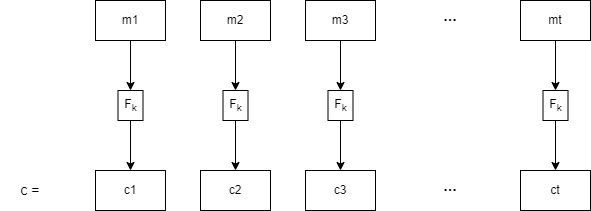
\includegraphics[width=0.8\textwidth]{ecb.jpg}
  \caption{ECB Mode Encryption}
\end{figure}
\\
\\ \textcolor{red}{This encryption mode is not secure}.
\begin{itemize}
    \item Same message block is encrypted to the same ciphertext block
    \begin{itemize}
    \item This implies that ECB is not CPA secure because it is stateless and deterministic.
    \end{itemize}
    \item If $F$ is PRF, we are not able to decrypt the ciphertext because it is not guaranteed that the inverse function of $F$ exists.
    \item If $F$ is PRP, we are able to decrypt the ciphertext but it is still not CPA secure because the same message still shares the same ciphertext.
\end{itemize}
\begin{figure}[h!]
  \centering
  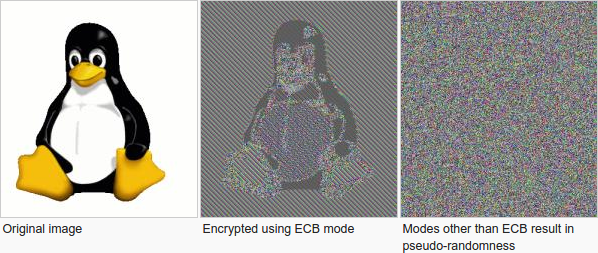
\includegraphics[width=0.5\textwidth]{figure4.png}
  \caption{ECB Encryption Example}
\end{figure}


%=============================================================================
%=============================================================================

\section{Pseudorandom Permutation (PRP)}


\subsection{Block cipher}
\begin{description}
    \item[Definition:] A keyed function $F$: $K$ x $\{0,1\}^{n} \rightarrow \{0,1\}^{n}$, where $F_{k}$ is bijection, and $F_{k}$ and $F_{k}^{-1}$ can be computed efficiently given the key k 
     \item[Note:] Block cipher is an invertible version of a PRF
\end{description}

\subsection{PRP}
\begin{description}
    \item[Definition:] $F_k$ is called a pseudorandom permutation (PRP) if $F_k$, given random key $k$ in key space $K$, is indistinguishable from a random bijection (permutation on $\{0,1\}^{n}$) for alll ppt A:
    \[
   \bigg| \Pr_{k \leftarrow{K}}\left[\cal A^{\text{$F_k(.)$}} = \text{1} \right] - \Pr_{P \leftarrow{P_n}}\left[\cal A^{\text{$P(.)$}} = \text{1}\right]\bigg| = negl(n)\]
  \[ \text{where $P_n$ is a set of all bijection on $\{0,1\}^{n}$}
  \]
  \item[Note:] If we can give A access to $F_k^{-1}(.)$/$P^{-1}(.)$ as well, then $F_k$ is a strong PRP.
  \item[Theorem:] If $F$ is a PRP, $F$ is also a PRF.
  \begin{description}
      \item[Proof Idea:] Given oracle access, a random permutation is identical to a random function as long as distinct input queries to the random function don't return the same value (because if $c_1=c_2$, function $F$ is not invertible), which implies "birthday collision" on outputs. However, collision happens with negligible probability: $\frac{poly(n)}{2^{n}}$. Thus, under the efficient setting, if $F$ is a PRP, it is also a PRF.
  \end{description}
\end{description}
%=============================================================================
%=============================================================================

\section{Cipher Block Chaining (CBC)}

\subsection{Encryption}
\begin{figure}[H]
  \centering
  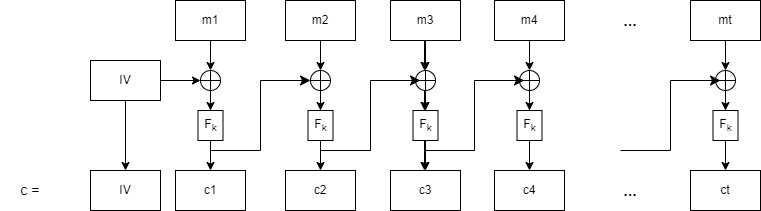
\includegraphics[width=0.8\textwidth]{cbc.jpg}
  \caption{CBC Mode Encryption}
\end{figure}
\begin{equation}
    \begin{cases}
      c_0 = IV\\
      c_i = F_k(m_i \oplus c_{i-1})
    \end{cases}
\end{equation}
\subsection{Decryption}
\begin{figure}[H]
  \centering
  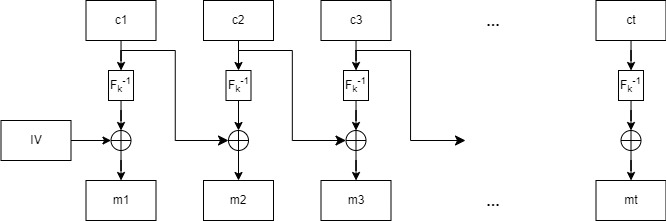
\includegraphics[width=0.8\textwidth]{cbc2.jpg}
  \caption{CBC Mode Decryption}
\end{figure}
\begin{equation}
      m_i = c_{i-1} \oplus F_k^{-1}(c_i)\\
\end{equation}
\begin{itemize}
    \item \textbf{Theorem:} If $F$ is a PRP (which is also PRF), then CBC is CPA-secure. 
    \begin{description}
        \item [Proof Idea:] All ciphertexts look like random independent strings as long as no input to $F_k(.)$ is ever repeated. Based on the birthday paradox, repetitions happen with only negligible ($\frac{poly(n)}{2^{n}}$) probability by the choice of IV and (pseudo)-random outputs of prior blocks.
    \end{description}
    \item \textbf{Cons}
\begin{enumerate}
    \item Longer execution time:
    \begin{itemize}
        \item Because we cannot trim the output of $F$ to fit the last message block, CBC requires padding the last message block which will increase the execution time.
    \end{itemize}
    \item Encryption is sequential
    \begin{itemize}
        \item Cannot compute ciphertext without computing all prior blocks
    \end{itemize}
    \begin{description}
        \item [Note:] Decryption can be done in parallel.
    \end{description}
    \item Can be broken in "streaming" contexts that fall slightly outside the CPA attack model
    \begin{itemize}
        \item \textbf{Padding Oracle Attack}: if attacker can get errors (padding error or encryption error) from CBC mode, the attacker can decrypt the entire message.
    \end{itemize}
\end{enumerate}
\end{itemize}



%=============================================================================
%=============================================================================

\bibliographystyle{alpha}
% Uncomment below if you have any references:
%\bibliography{\jobname}

%=============================================================================
%=============================================================================

\end{document}
